%% =============================================================
%%  Lire les notes — la portée, les clés, le do central
%%  Guide de référence, composé en LaTeX, gravures LilyPond
%% =============================================================
%%
%%  Les figures (gravures/l-*.cropped.pdf), le tableau des repères,
%%  la portée de onze lignes et les réponses des exercices
%%  (gravures/lecture-*.tex) sont produits par
%%  outils/generer_lecture.py, à partir du modèle de hauteurs des
%%  autres guides (outils/gammes.py). Voir le colophon en dernière page.
%%
\documentclass[a4paper,11pt]{article}

\usepackage[top=2.2cm,bottom=2.4cm,left=2.2cm,right=2.2cm]{geometry}
\usepackage[T1]{fontenc}
\usepackage[utf8]{inputenc}
\usepackage[french]{babel}
\usepackage{lmodern}
\usepackage{xcolor}
\usepackage{graphicx}
\usepackage{titlesec}
\usepackage{fancyhdr}
\usepackage{mdframed}
\usepackage{array}
\usepackage{enumitem}
\usepackage{booktabs}
\usepackage{tikz}
\usetikzlibrary{decorations.pathreplacing}
\usepackage{hyperref}

\graphicspath{{gravures/}}

% ---- Couleurs, reprises du document des accords de guitare ---------
\definecolor{navy}{RGB}{18,50,105}
\definecolor{lightnavy}{RGB}{235,241,255}
\definecolor{mygray}{RGB}{110,110,110}
\definecolor{accent}{RGB}{150,40,30}

\hypersetup{colorlinks=true, linkcolor=navy, urlcolor=navy,
  pdftitle={Lire les notes — la portée, les clés, le do central},
  pdfauthor={Fabian Bastin}}

% ---- En-tête et pied -----------------------------------------------
\pagestyle{fancy}
\fancyhf{}
\renewcommand{\headrulewidth}{0.4pt}
\renewcommand{\footrulewidth}{0.4pt}
\fancyhead[L]{\small\bfseries\textcolor{navy}{Lire les notes}}
\fancyhead[R]{\small\textcolor{mygray}{\thepage}}
\fancyfoot[C]{\small\textcolor{mygray}{La portée, les clés, le do central}}

% ---- Titres de section ---------------------------------------------
\newcommand{\navysect}[1]{%
  \colorbox{navy}{%
    \parbox[c][17pt]{\dimexpr\linewidth-2\fboxsep\relax}{%
      \color{white}\hspace{6pt}\bfseries\normalsize #1}}%
}
\titleformat{\section}[block]{\normalfont}{}{0pt}{\navysect}
\titlespacing*{\section}{0pt}{16pt}{10pt}

% ---- Encadré de remarque -------------------------------------------
\newmdenv[linecolor=navy, linewidth=0.5pt, backgroundcolor=lightnavy,
  innertopmargin=6pt, innerbottommargin=6pt,
  innerleftmargin=8pt, innerrightmargin=8pt,
  skipabove=8pt, skipbelow=8pt]{remarque}

% ---- Figure gravée ---------------------------------------------------
% Figure gravée, à la largeur donnée (part de la ligne), avec sa légende.
% Le tout tient dans une minipage : figure et légende ne sont jamais
% séparées par un saut de page.
\newcommand{\gravure}[3]{%
  \par\medskip\noindent
  \begin{minipage}{\linewidth}
    \centering
    \includegraphics[width=#2\linewidth]{#1.cropped.pdf}\\[4pt]
    {\small\itshape\color{mygray} #3}
  \end{minipage}\par\medskip
}

% Légende seule, sous une figure TikZ ou un tableau.
\newcommand{\legende}[1]{\\[4pt]{\small\itshape\color{mygray} #1}}

\setlist{itemsep=2pt, topsep=4pt, parsep=0pt}

\begin{document}

% =====================================================================
\begin{titlepage}
\centering
\vspace*{3cm}
{\Huge\bfseries\color{navy} Lire les notes\par}
\vspace{0.6cm}
{\LARGE\color{navy} La portée, les clés, le do central\par}
\vspace{1.4cm}
{\large De la position au nom\par}
\vspace{2.5cm}
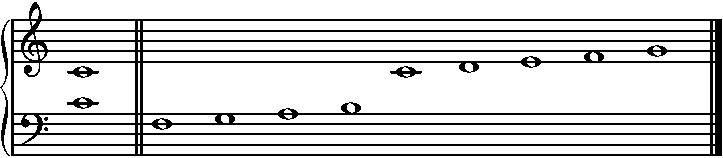
\includegraphics[width=0.6\linewidth]{l-grande-portee.cropped.pdf}
\vfill
{\small\color{mygray}
Gravures LilyPond, composition \LaTeX.\par}
\vspace{1cm}
\end{titlepage}

\tableofcontents
\newpage

% =====================================================================
\section{Avant-propos}

Une note s'écrit par sa position sur la portée, et la clé dit quelle note
occupe chaque position : elle en nomme une, les autres s'en déduisent en
comptant. Lire, c'est d'abord compter à partir de la clé, puis, à force de
repères, ne plus compter.

À lire avant
\href{https://www.slashbin.net/musique/theorie/intervalles.pdf}{\emph{Les
intervalles — du demi-ton à l'octave}}, qui suppose les notes connues en
clé~de~sol.

\begin{remarque}
\textbf{Conventions.} Les notes sont nommées en français : do, ré, mi, fa,
sol, la, si. Quand l'octave compte, un numéro suit le nom, à la française : le
do central du piano est le \emph{do3}, le do de l'octave au-dessus le do4. La
notation scientifique numérote un cran plus haut et l'écrit C4, mais certains
logiciels l'appellent C3 ;
\href{https://www.slashbin.net/musique/theorie/frequences.pdf}{\emph{Les
fréquences}} comparent ces usages.
\end{remarque}

% =====================================================================
\section{La portée}
\label{sec:portee}

\textbf{Cinq lignes, quatre interlignes.} La musique s'écrit sur une
\emph{portée} : cinq lignes horizontales, également espacées, et les quatre
espaces qui les séparent, les \emph{interlignes}. Les unes et les autres se
numérotent de bas en haut : la première ligne est la plus basse, le quatrième
interligne le plus haut.

\begin{center}
\begin{tikzpicture}[x=1cm, y=0.5cm, font=\small]
  \foreach \y/\rg in {0/1re, 1/2e, 2/3e, 3/4e, 4/5e} {
    \draw[line width=0.5pt] (0,\y) -- (6,\y);
    \node[right] at (6.15,\y) {\rg~ligne};
  }
  \foreach \y/\rg in {0/1er, 1/2e, 2/3e, 3/4e} {
    \node[left, mygray] at (-0.15,\y+0.5) {\rg~interligne};
  }
  \foreach \y/\rg in {5/1re, 6/2e} {
    \draw[accent, line width=0.5pt] (2.6,\y) -- (3.4,\y);
    \node[right, accent] at (3.55,\y) {\rg~ligne supplémentaire au-dessus};
  }
  \foreach \y/\rg in {-1/1re, -2/2e} {
    \draw[accent, line width=0.5pt] (2.6,\y) -- (3.4,\y);
    \node[right, accent] at (3.55,\y) {\rg~ligne supplémentaire au-dessous};
  }
\end{tikzpicture}
\legende{La portée. Lignes et interlignes se comptent de bas en haut ; les
lignes supplémentaires, en s'éloignant de la portée.}
\end{center}

\textbf{Chaque position est une note.} Une note s'écrit sur une ligne, que sa
tête traverse, ou dans un interligne, entre deux lignes. En montant, les
positions alternent : ligne, interligne, ligne… Passer d'une position à la
suivante, c'est passer d'une note à sa voisine. La portée en offre ainsi onze
sans rien ajouter : ses cinq lignes et ses quatre interlignes, plus une
position juste au-dessous de la première ligne et une juste au-dessus de la
cinquième.

\textbf{Les lignes supplémentaires.} Plus haut ou plus bas, on trace de
courtes lignes, le temps d'une note : les \emph{lignes supplémentaires}. Elles
se numérotent en s'éloignant de la portée --- la première au-dessus est la plus
proche de la cinquième ligne, la première au-dessous la plus proche de la
première ---, et les interlignes qu'elles délimitent de même. Au-delà de trois
ou quatre, elles se lisent mal : on change alors de clé
(section~\ref{sec:cles}).

% =====================================================================
\section{Les noms des notes}
\label{sec:noms}

\textbf{Sept noms, en cycle.} Les notes portent sept noms, toujours dans le
même ordre : do, ré, mi, fa, sol, la, si. Après si revient do, et le cycle
reprend. Monter d'une position sur la portée, c'est prendre le nom suivant ;
descendre, le précédent.

\gravure{l-sol-montee}{1}{En clé de sol, du do central au do deux octaves plus
haut : une position de plus, un nom de plus.}

\gravure{l-fa-descente}{1}{En clé de fa, du do central au do deux octaves plus
bas.}

\textbf{L'octave.} Sept positions plus haut --- huit notes en comptant celle de
départ, d'où son nom ---, le même nom revient : c'est l'\emph{octave}. Les deux notes sonnent si semblables que l'oreille les entend
comme une même note, l'une plus aiguë que l'autre. Le numéro qui suit le nom
distingue les octaves, et il change au do : do3, ré3… si3, puis do4. Sur la
portée, une note et son octave ne sont jamais toutes deux sur une ligne : sept
positions mènent d'une ligne à un interligne, et d'un interligne à une ligne.

\textbf{D'une ligne à la suivante.} Entre deux lignes voisines, on saute une
note : les lignes de la clé de sol portent mi, sol, si, ré, fa, et ses
interlignes fa, la, do, mi. Cette distance de trois noms, départ et arrivée
compris, est une \emph{tierce} ;
\href{https://www.slashbin.net/musique/theorie/intervalles.pdf}{\emph{Les
intervalles}} l'étudient avec les autres distances entre deux notes.

% =====================================================================
\section{Les clés}
\label{sec:cles}

Sans clé, la portée ne dit pas quelle note occupe quelle position. La
\emph{clé}, tracée au début de chaque ligne de musique, en fixe une : elle
donne son nom à la ligne sur laquelle elle est posée, et désigne une note
précise, dans une octave précise. Les autres positions s'en déduisent en
comptant.

\par\medskip\noindent
\begin{minipage}{\linewidth}
\centering
\begin{tabular*}{0.9\linewidth}{@{\extracolsep{\fill}}cccc@{}}
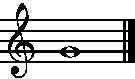
\includegraphics{l-cle-sol.cropped.pdf} &
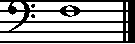
\includegraphics{l-cle-fa.cropped.pdf} &
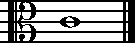
\includegraphics{l-cle-ut3.cropped.pdf} &
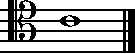
\includegraphics{l-cle-ut4.cropped.pdf} \\[2pt]
\small clé de sol & \small clé de fa & \small clé d'ut & \small clé d'ut \\
\small\color{mygray} sol3, 2\textsuperscript{e} ligne &
\small\color{mygray} fa2, 4\textsuperscript{e} ligne &
\small\color{mygray} do3, 3\textsuperscript{e} ligne &
\small\color{mygray} do3, 4\textsuperscript{e} ligne \\
\end{tabular*}
\legende{Ce que désigne chaque clé : la note et la ligne qui la porte. Les deux
clés d'ut désignent le même do, le do central.}
\end{minipage}\par\medskip

\textbf{La clé de sol} s'enroule autour de la deuxième ligne : cette ligne
porte le sol3, le premier sol au-dessus du do central. C'est la clé de l'aigu :
voix de femme et d'enfant, violon, flûte, main droite du piano.

\textbf{La clé de fa} pose ses deux points de part et d'autre de la quatrième
ligne : cette ligne porte le fa2, le premier fa au-dessous du do central. C'est
la clé du grave : voix de basse et de baryton, violoncelle, contrebasse,
basson, main gauche du piano.

\textbf{Les clés d'ut} désignent le do central lui-même, sur la ligne qu'elles
encadrent : la troisième pour l'alto, la quatrième pour l'aigu du violoncelle,
du basson ou du trombone. Elles épargnent les lignes supplémentaires aux
instruments dont l'étendue se trouve entre les deux clés principales.

% =====================================================================
\section{Le do central et la grande portée}
\label{sec:do}

\textbf{Le do central.} Le do le plus proche du milieu du clavier s'appelle le
\emph{do central} : c'est le do3. Il tombe entre les deux clés principales :
sur la première ligne supplémentaire au-dessous en clé de sol, sur la première
au-dessus en clé de fa.

\textbf{Une portée de onze lignes.} Les cinq lignes de la clé de fa, la ligne
du do central et les cinq lignes de la clé de sol forment ensemble une seule
portée de onze lignes, toutes à une tierce l'une de l'autre. La musique pour
piano en garde les deux groupes de cinq et ne trace la ligne du milieu qu'en
ligne supplémentaire, quand une note s'y pose. Le sol3 de la clé de sol est
deux lignes au-dessus du do central, le fa2 de la clé de fa deux lignes
au-dessous.

\begin{center}
%% Produit par outils/generer_lecture.py — ne pas modifier à la main.
\begin{tikzpicture}[x=1cm, y=0.45cm]
  \draw[line width=0.5pt] (0,0) -- (6,0);
  \node[right, font=\small] at (6.3,0) {sol1};
  \draw[line width=0.5pt] (0,1) -- (6,1);
  \node[right, font=\small] at (6.3,1) {si1};
  \draw[line width=0.5pt] (0,2) -- (6,2);
  \node[right, font=\small] at (6.3,2) {ré2};
  \draw[line width=0.5pt] (0,3) -- (6,3);
  \node[right, font=\small] at (6.3,3) {fa2};
  \draw[line width=0.5pt] (0,4) -- (6,4);
  \node[right, font=\small] at (6.3,4) {la2};
  \draw[accent, dashed, line width=0.7pt] (2.2,5) -- (3.8,5);
  \node[right, accent, font=\small\bfseries] at (6.3,5) {do3, le do central};
  \draw[line width=0.5pt] (0,6) -- (6,6);
  \node[right, font=\small] at (6.3,6) {mi3};
  \draw[line width=0.5pt] (0,7) -- (6,7);
  \node[right, font=\small] at (6.3,7) {sol3};
  \draw[line width=0.5pt] (0,8) -- (6,8);
  \node[right, font=\small] at (6.3,8) {si3};
  \draw[line width=0.5pt] (0,9) -- (6,9);
  \node[right, font=\small] at (6.3,9) {ré4};
  \draw[line width=0.5pt] (0,10) -- (6,10);
  \node[right, font=\small] at (6.3,10) {fa4};
  \draw[navy, decorate, decoration={brace, amplitude=5pt}] (-0.25,6) -- (-0.25,10) node[midway, left=7pt, font=\small, navy] {clé de sol};
  \draw[navy, decorate, decoration={brace, amplitude=5pt}] (-0.25,0) -- (-0.25,4) node[midway, left=7pt, font=\small, navy] {clé de fa};
\end{tikzpicture}

\legende{Les onze lignes de la grande portée. En pointillé, la ligne du do
central, tracée seulement quand une note s'y pose.}
\end{center}

\textbf{L'accolade.} Quand un instrument lit les deux clés à la fois ---
piano, harpe, orgue ---, ses deux portées sont reliées par une
\emph{accolade} : la clé de sol en haut, pour la main droite, la clé de fa en
bas, pour la main gauche. Le do central appartient aux deux portées ; on
l'écrit dans celle de la main qui le joue.

\gravure{l-grande-portee}{0.75}{Le do central, écrit dans chaque portée, puis
une gamme de fa2 à sol3 qui passe de la clé de fa à la clé de sol.}

% =====================================================================
\section{Lire sans compter}
\label{sec:reperes}

Compter à partir de la clé fonctionne toujours, mais lentement. Quelques
repères suffisent bientôt.

\begin{center}
%% Produit par outils/generer_lecture.py — ne pas modifier à la main.
\begin{tabular}{@{}l *{5}{c} @{\hspace{14pt}} *{4}{c}@{}}
\toprule
 & \multicolumn{5}{c}{\textbf{Lignes}} & \multicolumn{4}{c}{\textbf{Interlignes}} \\
\cmidrule(lr){2-6}\cmidrule(l){7-10}
 & 1 & 2 & 3 & 4 & 5 & 1 & 2 & 3 & 4 \\
\midrule
Clé de sol & mi3 & sol3 & si3 & ré4 & fa4 & fa3 & la3 & do4 & mi4 \\
Clé de fa & sol1 & si1 & ré2 & fa2 & la2 & la1 & do2 & mi2 & sol2 \\
\bottomrule
\end{tabular}

\legende{Les notes des lignes et des interlignes, dans les deux clés.}
\end{center}

\textbf{Trois do.} Le do central, sur la première ligne supplémentaire, dans
les deux clés ; le do4, au troisième interligne de la clé de sol ; le do2, au
deuxième interligne de la clé de fa. Les deux derniers sont à une octave du do
central, de part et d'autre.

\textbf{D'une clé à l'autre.} À position égale, la clé de fa nomme la note
deux noms plus loin que la clé de sol : la première ligne, mi en clé de sol,
est sol en clé de fa ; le deuxième interligne, la en clé de sol, est do en clé
de fa. La note est aussi bien plus grave, de près de deux octaves.

% =====================================================================
% Une page à part : sans ce saut, le titre et sa phrase restaient seuls en bas
% de page, les deux portées d'exercices sur la suivante.
\clearpage
\section{S'exercer}
\label{sec:exercices}

Les notes ci-dessous sont à nommer, avec leur numéro d'octave. Les réponses
suivent.

\gravure{l-exercice-sol}{1}{En clé de sol.}

\gravure{l-exercice-fa}{1}{En clé de fa.}

\begin{remarque}
\textbf{Réponses.}

%% Produit par outils/generer_lecture.py — ne pas modifier à la main.
\textbf{En clé de sol.} 1~:~sol3, 2~:~do4, 3~:~do3, 4~:~fa4, 5~:~mi3, 6~:~ré4, 7~:~la3, 8~:~la4, 9~:~ré3, 10~:~mi4, 11~:~si3, 12~:~do5.

\textbf{En clé de fa.} 1~:~fa2, 2~:~do2, 3~:~do3, 4~:~sol1, 5~:~la2, 6~:~mi1, 7~:~mi2, 8~:~la1, 9~:~mi3, 10~:~ré2, 11~:~sol2, 12~:~fa1.

\end{remarque}

% =====================================================================
\section*{Colophon}
\addcontentsline{toc}{section}{Colophon}

Les gravures musicales sont produites par \textbf{LilyPond}, la composition
par \textbf{\LaTeX}. Les figures, le tableau des repères, la portée de onze
lignes et les réponses des exercices dérivent du modèle de hauteurs des autres
guides, le module \texttt{gammes.py} du dossier \texttt{outils}, et d'une seule
donnée par clé : la ligne qu'elle désigne et la note qu'elle y place. Avant
d'écrire quoi que ce soit, le générateur vérifie ce que le texte affirme : la
place du do central dans chaque clé, les onze lignes de la grande portée,
l'écart de deux noms entre les deux clés. Pour régénérer l'ensemble :

\begin{center}
\texttt{python3 outils/generer\_lecture.py}\\
\texttt{lilypond -dcrop --formats=pdf gravures/l-*.ly}\\
\texttt{pdflatex lecture.tex}
\end{center}

\end{document}
